\documentclass{article}
\usepackage[utf8]{inputenc}
\usepackage{graphicx}
\graphicspath{ {images/}}
\usepackage{wrapfig}
\usepackage{fancyvrb}
 
\title{TP3}
\author{RAJA GANAPATHY Srinivas ENGUIX Précillia}


\begin{document}
\maketitle
        
\section{Exemple}
$$ $$

Nous savons que l'équation différentielle ordinaire est de la forme u'(t) = f(t,u(t)) et u(0) = u0. Pour cet exemple, nous avons une équation différentielle ordinaire très simple, nous avons u'(t) = - u(t) et u(0) = 1.0. Ici, la fonction f vaut - u(t). A la l'aide du module "matplotlib" nous avons pu représenter graphiquement u: 

\begin{wrapfigure}{l}{1\textwidth}
        \centering
        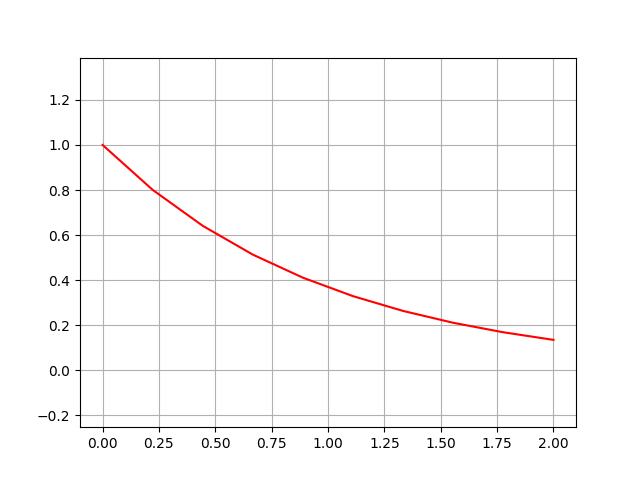
\includegraphics[width=0.75\textwidth]{graph1.png}
       
\end{wrapfigure}

$$ $$
$$ $$
$$ $$
$$ $$
$$ $$
$$ $$
$$ $$
$$ $$
$$ $$
$$ $$
$$ $$

\section{Méthode d'Euler}
$$ $$

Nous avons un intervalle donné [0,T], pour obtenir un calcul approché de u au moyen de la méthode d'Euler, on divise tout d'abord l'intervalle [0,T] en n parties égales. Puis on pose h = T/n, on obtient donc une subdivision. A partir de là, on peut calculer approximativement la valeur de u aux points tk de la subdivision. On a d'abord calculé les n+1 premiers termes de la suite (uk), défini par la méthode d'Euler. Nous avons ensuite représenté sur le même graphique la solution exacte u et les points (tk,uk):

\begin{wrapfigure}{l}{1\textwidth}
        \centering
        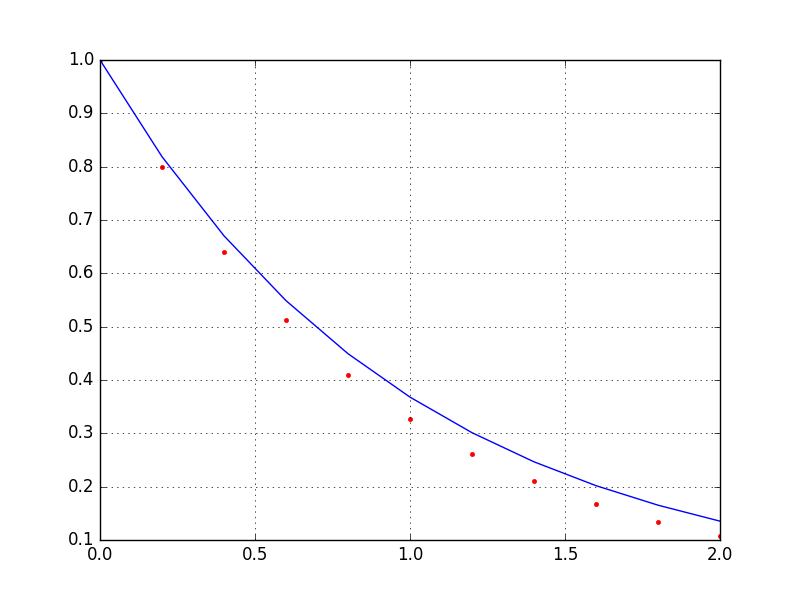
\includegraphics[width=0.75\textwidth]{graph2.png}
       
\end{wrapfigure}

$$ $$
$$ $$
$$ $$
$$ $$
$$ $$
$$ $$
$$ $$
$$ $$
$$ $$
$$ $$
$$ $$

\section{Fonction Euler}
$$ $$

La fonction Euler prend en argument une fonction python f, de deux variables scalaires t et u, une valeur initiale u0, un réel T, un entier n, et qui renvoie deux numpy arrays (converties les données numériques en tableaux); tt de taille n+1, contenant les valeurs tk, obtenues par la méthode d'Euler et uu de taille n+1, contenant les valeurs uk, obtenues par la méthode d'Euler.

$$ $$
$$ $$

\section{Application de la fonction Euler}
$$ $$

Pour commencer nous avons écrit la fonction f qui était dans l'exemple 2, la fonction f donne en python :
\newline
\newline
\begin{wrapfigure}{l}{1\textwidth}
        \centering
        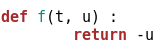
\includegraphics[width=0.25\textwidth]{f.png}
\end{wrapfigure}

$$ $$
$$ $$

On a ensuite appliqué la fonction Euler à l'exemple 2 et on a retrouvé les mêmes résultats que ceux de l'exemple 2.
\newline
Ensuite on devait examiner les équations différentielles ordinaires suivantes :
\newline
\newline
\begin{wrapfigure}{l}{1\textwidth}
        \centering
        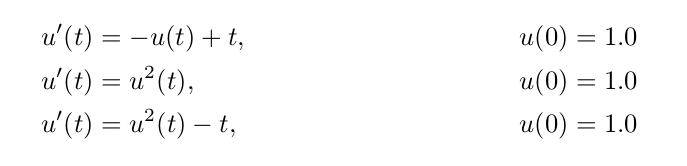
\includegraphics[width=0.75\textwidth]{edo.png}
\end{wrapfigure}

$$ $$
$$ $$
$$ $$
$$ $$

On a calculé les deux premières équations différentielles à la main (voir la copie rendue en cours). A contrario, la troisième EDO ne peut pas être calculé à la main, car le calcul devient tout de suite trop compliqué.

$$ $$

\section{Intégration d'une EDO d'ordre supérieur}
 
$$ $$

Nous allons maintenant montrer comment intégrer une EDO d'ordre supérieur. On prend l'exemple de l'oscillateur harmonique (modélisation du ressort) qui est une EDO d'ordre 2 : 
\newline
\begin{wrapfigure}{l}{1\textwidth}
        \centering
        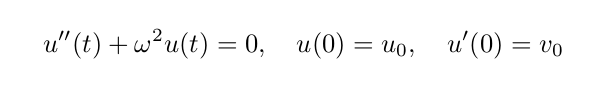
\includegraphics[width=0.75\textwidth]{e2.png}
\end{wrapfigure}

$$ $$

Ici, w, u0, v0, sont des scalaires donnés; w s'appelle la pulsation, u0 la position initiale, et v0 la vitesse initiale. Posons ensuite v = u' et écrivons l'EDO sous la forme :
\newline
\begin{wrapfigure}{l}{1\textwidth}
        \centering
        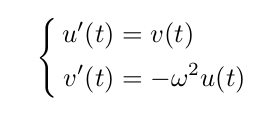
\includegraphics[width=0.35\textwidth]{e3.png}
\end{wrapfigure}

$$ $$
$$ $$

On a ensuite calculé la solution exacte de l'EDO 4 (voir la copie rendu en cours). Nous avons ensuite écrit la fontion F de l'EDO 5 dans une fonction python F; on choisira w = 1.0, F prendra en arguments un flottant t et un numpy array U de taille 2.
\newline
\newline
Nous avons modifié la fonction Euler, pour qu'elle prenne 4 arguments: une fonction python F (elle même prenant 2 arguments t flottant et U numpy array de taille 2), une valeur initiale U0 numpy array, un flottant T et un entier n; Euler renverra 2 numpy arrays : tt de taille n+1, contenant les valeurs tk, et UU de taille 2*(n+1), contenant les valeus Uk obtenues par la méthode d'Euler.
\newline
\newline
Voici les 2 fonctions Euler pour constater les modifications de la fonction de base:
\newline
\begin{wrapfigure}{l}{1\textwidth}
        \centering
        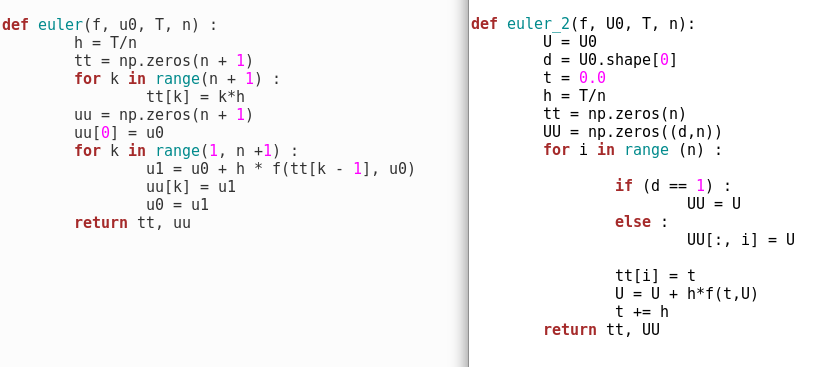
\includegraphics[width=1\textwidth]{e4.png}
\end{wrapfigure}

$$ $$
$$ $$
$$ $$
$$ $$
$$ $$
$$ $$
$$ $$
$$ $$

Nous avons résolu par la suite l'EDO 4, avec w = 1.0, T = 4$\pi$ et les conditions initiales u(0) = 1.0, u'(0) = 0.0. Nous avons essayé différentes valeurs de n.
\newline
\newline
Pour finir, nous avons représenté graphiquement la position u en fonction du temps t, la vitesse v en fonction du temps t, et la vitesse v en fonction de la position u.
\newline
Voici ce graphique ci-dessous:
\newline
\begin{wrapfigure}{l}{1\textwidth}
        \centering
        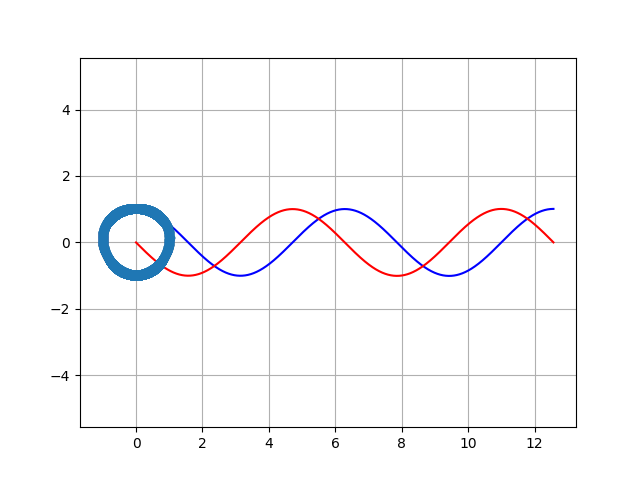
\includegraphics[width=1\textwidth]{graphf5.png}
\end{wrapfigure}

$$ $$
$$ $$
$$ $$
$$ $$
$$ $$
$$ $$
$$ $$
$$ $$
$$ $$
$$ $$
$$ $$
$$ $$
$$ $$
$$ $$
$$ $$

\section{Analyse de la séance de TP}
$$ $$

Nous avons trouvé ce TP moins long au niveau du codage mais tout aussi long au niveau du latex. Les calculs manuel des EDO nous ont pris beaucoup de temps. Nous constatons que nous avons de plus en plus de facilité à coder en python.







\end{document}
